% 四阶龙格库塔法

\pentry{中点法解常微分方程(组)\upref{OdeMid}}

\textbf{龙格库塔法} 是一类数值解微分方程的算法, 其中较常见的是\textbf{四阶龙格库塔法}. 这里不进行推导, 仅仅给出公式如下($y_n, t_n, h$ 的定义类比\autoref{OdeNum_eq5}\upref{OdeNum})
\begin{equation}\label{OdeRK4_eq1}
y_{n+1} = y_n + \frac h6 (k_1 + 2k_2 + 2k_3 + k_4)
\end{equation}
其中
\begin{equation}\label{OdeRK4_eq2}
\ali{
k_1 &= f(y_n, t_n) 
& k_2 &= f\left(y_n + h\frac{k_1}{2}, t_n + \frac h2 \right)\\
k_3 &= f\left( y_n + h\frac{k_2}{2}, t_n + \frac h2\right) \qquad
&k_4 &= f(y_n + hk_3, t_n + h)
}\end{equation}
由以上两式, 不难把该算法拓展到方程组的情况. 对于 $N$ 元微分方程组
\begin{equation}\leftgroup{
y'_1(t) &= f_1(y_1,\dots, y_N, t)\\
y'_2(t) &= f_2(y_1,\dots, y_N, t)\\
& \vdots\\
y'_N(t) &= f_N(y_1,\dots, y_N, t)
}\end{equation}
我们可以把该式记为矢量函数的形式
\begin{equation}\label{OdeRK4_eq4}
\vec y'(t) = \vec f(\vec y, t)
\end{equation}
现在我们仅需要把\autoref{OdeRK4_eq1} 和 \autoref{OdeRK4_eq2} 中的所有 $y_i$ 和 $k_i$ 都变为 $N$ 维列矢量 $\vec y_i$ 和 $\vec k_i$ 即可将微分方程拓展为微分方程组.

\subsection{例程}

到目前为止, 我们每求一个微分方程的数值解都要重新写一次程序, 对于一些较为复杂的算法这样做效率较低. 我们这里不妨把四阶龙格库塔法写到一个单独的函数文件 odeRK4.m 中, 当我们要解某个特定的方程时, 只需把\autoref{OdeRK4_eq2} 中的 $f(y, t)$ 作为自变量输入即可解出 $y(t)$.

\subsubsection{odeRK4.m}
\begin{lstlisting}[language=Matlab]
function [Y, t] = odeRK4(f, tspan, Y0, Nt)
Nvar = numel(Y0);  % 因变量的个数
dt = (tspan(2) - tspan(1)) / (Nt-1); % 计算步长
Y = zeros(Nvar, Nt);
Y(:, 1) = Y0(:);
t = linspace(tspan(1), tspan(2), Nt);

for ii=1:Nt-1
    K1 = f( t(ii),        Y(:,ii)          );
    K2 = f( t(ii)+dt/2,   Y(:,ii)+K1*dt/2  );
    K3 = f( t(ii)+dt/2,   Y(:,ii)+K2*dt/2  );
    K4 = f( t(ii)+dt,     Y(:,ii)+K3*dt    );
    Y(:,ii+1) = Y(:,ii) + dt/6 * (K1+2*K2+2*K3+K4);
end
end
\end{lstlisting}

我们先来看第 1 行的函数声明, 输入变量中,\texttt{f} 是\autoref{OdeRK4_eq4} 中 $\vec f(\vec y, t)$ 的函数句柄\upref{MatFun}, \texttt{tspan} 是一个 $2\times1$ 的列矢量, \texttt{tspan(1)} 是初始时间, \texttt{tspan(2)} 是终止时间, \texttt{Y0} 是一个列矢量, \texttt{Y0(ii)} 是第 \texttt{ii} 个因变量的初始值, \texttt{Nt} 是 $t_n$ 的个数, \texttt{tspan} 定义的时间区间被等分为 \texttt{Nt - 1} 个小区间. 因变量中, \texttt{Y} 的行数是因变量的个数, 列数是 \texttt{Nt}, \texttt{t} 是一个行矢量, 由第 6 行定义, \texttt{Y(ii, jj)} 就是第 \texttt{ii} 个变量在 \texttt{t(jj)} 时刻的值. 第 5 行把初值 \texttt{Y0} 赋给 \texttt{Y} 的第 1 列, 第 8-14 行的循环根据\autoref{OdeRK4_eq1} 和\autoref{OdeRK4_eq2} 的矢量形式由 \texttt{Y} 的第 \texttt{ii} 列($\vec y_i$)求第 \texttt{ii+1} 列($\vec y_{i+1}$).

我们先来用这个函数来计算“天体运动的简单数值计算\upref{KPNum0}” 中的问题. 我们令因变量 $\vec y$ 的四个分量依次为一阶方程组(\autoref{OdeNum_eq4}\upref{OdeNum})
\begin{equation}\label{OdeRK4_eq5}
\leftgroup{
x' &= v_x\\
y' &= v_y\\
v'_x &= -GMx/(x^2 + y^2)^{3/2}\\
v'_y &= -GMy/(x^2 + y^2)^{3/2}
}\end{equation}
中的 $x, y, v_x, v_y$. 程序代码如下

\subsubsection{KeplerRK4.m}
\Matlab
function KeplerRK4
% 参数设定
GM = 1; % 万有引力常数乘以中心天体质量
x0 = 1; y0 = 0; % 初始位置
vx0 = 0; vy0 = 0.7; % 初始速度
tspan = [0; 4]; % 总时间和步数
Nt = 100; % 步数

Y0 = [x0; y0; vx0; vy0]; % 因变量初值
f = @(Y, t)fun(Y, t, GM);
[Y,~] = odeRK4(f, tspan, Y0, Nt);

% 画图
figure; hold on;
plot(Y(1,:), Y(2,:));
scatter(0, 0);
axis equal;
end

function Y1 = fun(Y, ~, GM)
% 因变量
x = Y(1); y = Y(2);
vx = Y(3); vy = Y(4);
Y1 = zeros(4,1); % 预赋值
Y1(1) = vx;
Y1(2) = vy;
temp = -GM /(x^2 + y^2)^(3/2);
Y1(3) = temp * x;
Y1(4) = temp * y;
end
\end{lstlisting}

运行结果如\autoref{OdeRK4_fig1} 所示.

\begin{figure}[ht]
\centering
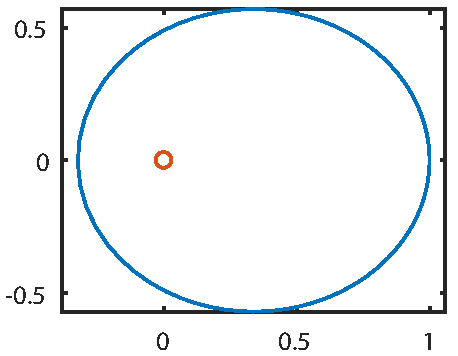
\includegraphics[width=7cm]{./figures/OdeRK4.pdf}
\caption{运行结果} \label{OdeRK4_fig1}
\end{figure}

我们先来看函数 \texttt{fun} (20 行), 这个函数就相当于\autoref{OdeRK4_eq5}. 第一个输入变量 \texttt{Y} 是一个列矢量, 是 $\vec y_n$ 的值, 第二个输入变量是 $t$, 但由于\autoref{OdeRK4_eq5} 中没有出现 $t$, 我们用波浪线代替. 第三个输入变量是参数 $GM$, 即万有引力常数和中心天体质量之积. 输出变量 \texttt{Y1} 是一个列矢量, 是 $\vec y'_n$ 的值.

再来看主函数 \texttt{KeplerRK4} (第 1 行), 参数设定中除了步数从 4000 变为了 100, 其他都和“天体运动的简单数值计算\upref{KPNum0}” 中的程序一样, 然而这里运行结果却精确得多(曲线几乎闭合), 可见这种算法的优越性.

主函数第 10 行中将 \texttt{fun(Y, t, GM)} 变为函数句柄 \texttt{f(Y, t)}, 这样 \texttt{GM} 就可以在“参数设定” 中设置, 而不用在 \texttt{fun} 函数内部设置. 第 11 行调用了上文中的 \texttt{odeRK4} 函数解方程组, 由于我们在画图时不需要用 \texttt{t}, 所以把第二个输出变量改为波浪线.
